\documentclass[../main.tex]{subfile}
\graphicspath{{\subfix{../images}}}
\begin{document}

目标检测是计算机视觉中一项基本但具有挑战性的任务,它需要算法为图像中的每个感兴趣的实例预测带有类别标签的边界框。目前所有主流检测器如Faster R-CNN\cite{fasterrcnn}、SSD\cite{ssd}和YOLOv2、v3\cite{yolov3}都依赖于一组预定义的锚框,长期以来一直认为\textit{使用锚框是检测器成功的关键}。尽管取得了巨大的成功,但重要的是要注意基于锚的检测器有一些缺点:1) 如 [15, 24] 所示,检测性能对锚框的大小、长宽比和数量很敏感。例如,在 RetinaNet\cite{retinanet}中,改变这些超参数最多可以在 COCO 基准测试上影响 4\% 的AP [16]。因此,需要在基于锚的检测器中仔细调整这些超参数。 2)即使经过精心设计,由于锚框的尺度和纵横比保持固定,检测器在处理具有较大形状变化的候选对象时遇到困难,尤其是对于小对象。预定义的锚框也阻碍了检测器的泛化能力,因为它们需要在具有不同对象大小或长宽比的新检测任务上重新设计。 3)为了实现高召回率,一个基于锚的检测器需要在输入图像上密集放置锚框(例如,对于短边为800的图像,特征金字塔网络(FPN)\cite{fpn}中存在超过180K个锚框)。大多数这些锚框在训练期间被标记为负样本。过多的负样本加剧了训练中正负样本的不平衡。 4) 锚框还涉及复杂的计算,例如使用ground-truth边界框计算 IoU 分数。

最近,全卷积网络 (FCN) \cite{fcn} 在语义分割 [20、28、9、19]、深度估计 [17、31]、关键点检测 [3] 和计数 [2] 等密集预测任务中取得了巨大成功。作为高级视觉任务之一,目标检测可能是唯一一个偏离整洁的全卷积每像素预测框架的任务,主要是由于使用了锚框。提出一个问题是很自然的:\textit{我们能否以简洁的每像素预测方式解决对象检测,例如,类似于语义分割的 FCN?}因此,这些基本的视觉任务可以(几乎)统一在一个框架中。我们证明答案是肯定的。此外,我们首次证明,更简单的基于 FCN 的检测器比基于锚的检测器实现了更好的性能。

\begin{figure}[htb]
    \centering
    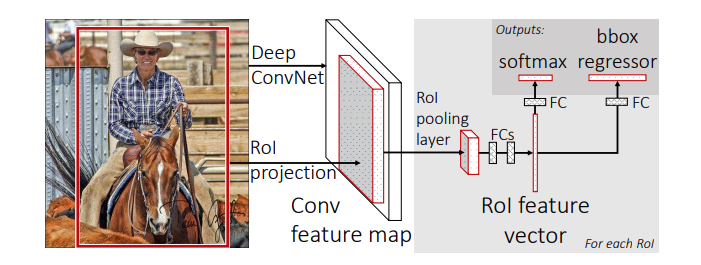
\includegraphics[width=\textwidth]{fig1.png}
    \caption{如左图所示,FCOS 通过预测 4D 向量$\left(l,t,r,b\right)$对每个前景像素的边界框位置进行编码(在训练期间由ground-truth边界框信息监督)。 右图显示,当一个位置在多个边界框中时,该位置应该回归哪个边界框可能不明确。}
    \label{fig:fig1}
\end{figure}

在文献中,一些工作尝试利用基于 FCN 的框架进行对象检测,例如 DenseBox\cite{densebox}。具体来说,这些基于 FCN 的框架直接在每个特征图层级上的每个空间位置预测 4D 向量和类别。如图\ref{fig:fig1}(左)所示,4D 向量描绘了从边界框的四个边到该位置的相对偏移量。这些框架类似于用于语义分割的 FCN,不同之处在于每个位置都需要回归 4D 连续向量。然而,为了处理不同大小的边界框,DenseBox\cite{densebox}将训练图像裁剪和调整到固定尺寸。因此 DenseBox 必须对图像金字塔进行检测,这违背了 FCN 一次计算所有卷积的理念。此外,更重要的是,这些方法主要用于特殊领域的物体检测,例如场景文本检测 [33, 10] 或人脸检测 [32, 12],因为人们认为这些方法在应用于可能高度重叠的通用物体检测时效果不佳。如图 1(右)所示,高度重叠的边界框导致难以处理的歧义:不清楚 w.r.t.重叠区域中的像素应该回归哪个边界框。

在续集中,我们仔细研究了这个问题,并表明使用 FPN 可以在很大程度上消除这种歧义。因此,我们的方法已经可以获得与那些传统的基于锚的检测器相当的检测精度。此外,我们观察到我们的方法可能会在远离目标对象中心的位置产生许多低质量的预测边界框。为了抑制这些低质量的检测,我们引入了一个新的“中心度”分支(只有一层)来预测像素与其相应边界框中心的偏差,如方程\ref{equ:centerness}中所定义。然后使用该分数降低检测到的低质量边界框的权重,并在 NMS 中合并检测结果。简单而有效的中心分支使得基于 FCN 的检测器在完全相同的训练和测试设置下优于基于锚的检测器。

这个新检测框架有如下优势。

\begin{itemize}
    \item 检测现在与许多其他可以使用FCN解决的任务(例如语义分割)统一起来,从而更容易重用这些任务中的想法。
    \item 检测不再需要候选和锚框,这显着减少了设计参数的数量。 设计参数通常需要启发式调整,并涉及许多技巧以实现良好的性能。 因此,我们的新检测框架使检测器,尤其是其训练变得更加简单。
    \item 通过消除锚框,我们的新检测器完全避免了与锚框相关的复杂计算,例如训练期间锚框与真实框之间的 IOU 计算和匹配。从而相对于基于锚的对应检测器,实现更快的训练和测试以及更少的训练内存占用。
    \item 没有花里胡哨,我们在单阶段检测器中实现了最好的结果。 我们还表明,所提出的 FCOS 可以用作两阶段检测器中的区域候选网络 (RPN),并且可以实现比基于锚的 RPN 对应物明显更好的性能。 鉴于更简单的无锚检测器的性能甚至更好,我们鼓励社区重新考虑锚框在目标检测中的必要性,它目前被认为是事实上的检测标准。
    \item 所提出的检测器可以立即以最少的修改扩展到其他视觉任务,包括实例分割和关键点检测。 我们相信这种新方法可以成为许多实例预测问题的新基线。
\end{itemize}

\end{document}